\documentclass[]{aiaa-tc} % insert '[draft]' option to show overfull boxes

 \title{Gradient-Based Optimization on Large Design Spaces with Graph-Based Problem Formulation In OpenMDAO}

\author{
  Tristan A. Hearn,%
     \thanks{Aerospace Engineer, MDAO Branch, Mail Stop 5-10, AIAA Member}
  \ Kenneth T. Moore,%
     \thanks{Senior Systems Engineer, MDAO Branch, Mail Stop 500-105, AIAA Senior Member}
  \ Justin Gray,%
     \thanks{Aerospace Engineer, MDAO Branch, Mail Stop 5-11, AIAA Member}
   \\
  {\normalsize\itshape
  NASA Glenn Research Center, Cleveland, OH}  \\
 }

\AIAAconference{Multidisciplinary Design Optimization Specialist Conference}
\AIAAcopyright{\AIAAcopyrightD{2012}}


% Define commands to assure consistent treatment throughout document
\newcommand{\eqnref}[1]{(\ref{#1})}
\newcommand{\class}[1]{\texttt{#1}}
\newcommand{\package}[1]{\texttt{#1}}
\newcommand{\file}[1]{\texttt{#1}}
\newcommand{\BibTeX}{\textsc{Bib}\TeX}

\setlength{\abovecaptionskip}{0pt}
\setlength{\belowcaptionskip}{0pt}

\usepackage{setspace}

\usepackage{graphicx}
\usepackage{wrapfig}
\usepackage{caption}
\usepackage{amsmath}
\usepackage{lscape}
\usepackage{hyperref}
\usepackage{minted}
\usepackage{color}
\usepackage{appendix}
\usepackage[section]{placeins}

\newcommand{\txt}{\textrm}


\captionsetup[figure]{margin=5pt,font=small,labelfont=bf,textfont=bf,justification=justified,}
%\captionsetup[wrapfigure]{margin=5pt,font=small,labelfont=bf,justification=justified,singlelinecheck=off}
\captionsetup[table]{margin=5pt,font=small,labelfont=bf,textfont=bf,justification=justified,position=top}

\bibliographystyle{aiaa}

\usepackage{lettrine}
\usepackage{verbatim}

\begin{document}

  \maketitle

  \begin{abstract}

  \end{abstract}

  \section{Introduction}

    Many of today's the most interesting design problems involve very large design spaces with 100's or 1000's of
    design variables. Large design spaces are often approached through the use of gradient based optimization
    analytic derivatives to achieve highly scalable solution strategies. For instance, adjoint based gradient
    methods have allowed CFD based shape optimization to tackle problems with 100's of design variables. [Cite Juan's Groups

    work here]. Coupled Aero-structural optimization is another area where gradient based optimization methods have
    been employed. [Cite Martins groups work here]. Although these problems have large design spaces,
    they include only a few disciplines (i.e. Geometry, Aerodynamics, Structures). The relative simplicity of
    the problem formulation make it feasible to use custom implementations tailored to a specific problem. Naturally however,
    this approach also limits the problem complexity that can be addressed with current MDAO methods.

    On the other end of the spectrum, traditional systems analysis models can be composed of 10's to 100's of disciplines,
    but usually work with lower fidelity analyses. These problems commonly contain a very high degree of interdisciplinary
    coupling, while working with lower fidelity analyses. These more complex problem formulations are much more difficult to compute
    analytic derivatives for at the system level, even if each discipline could provide its own partial derivatives. So many
    problems are solved using a finite difference approach, which restricts the size of the design space.

    If you placed complexity on the Y-axis and Fidelity on the X-axis, then the problem spectrum resemble the notional
    cartoon in Figure \ref{fig:complexity_cartoon}. In this diagram, there is a gap between the lower and higher fidelity
    type problems is indicative of the bifurcation in methods used to solve each type of problem currently. This gap begs the
    question, ``How should you appraoch a problem of medium complexity and medium fidelity?'' We propose that the answer to this
    dilemma is to develop a more general manner of implementing MDAO problems that can be applied to any problem across the entire
    space of complexity and fidelity.

    \begin{figure}[!htb]\begin{center}
      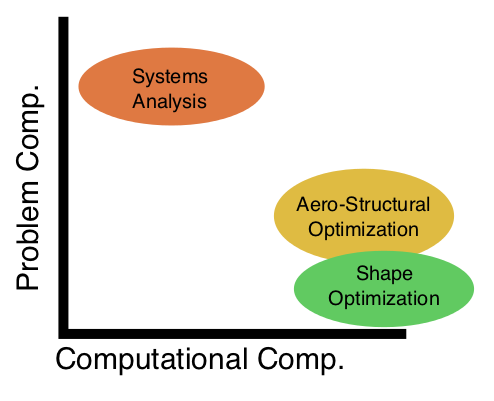
\includegraphics[width=.5\textwidth]{images/complexity_cartoon}
      \caption{ Notional spectrum of design problems currently being addressed. \label{fig:complexity_cartoon}}
    \end{center}\end{figure}

    In this work we demonstrate how OpenMDAO, an open-source framework, such a general
    solution to constructing and solving complex problems with large design spaces using the
    same MDAO methods commonly applied to the the shape optimization and aero-structural optimization
    problems. OpenMDAO achieves this by providing three key features:

    \begin{enumerate}
      \item Automatic handling of arbitrary interdisciplinary coupling
      \item Automatic formulation of gradients, including coupled derivatives, given arbitrary coupling
      \item Efficient operation in a high performance computing environment with distributed data
    \end{enumerate}

    \begin{comment}
      \begin{enumerate}
        \item Combining analytic derivatives with finite difference in a mixed derivatives environment
        \item Efficient solving for the coupled derivatives at the system level
        \item Assembly of the full gradient from the partial derivatives of each discipline
        \item Flexbility via separation of problem formulation from solution strategy
        \item Simple implementation for multi-point design problems
      \end{enumerate}
    \end{comment}

    To demonstrate these capabilities, we present two different problems representing different levels of
    complexity and fidelity, solved within the OpenMDAO framework. The fist problem is the design of a small
    satellite platform for taking weather measurements in the thermosphere, called CADRE. The CADRE problem has a
    complex problem formulation with XX disciplines and over 25000 design variables, but is lower fidelity and can
    be run on a single processor. This problem demonstrates that OpenMDAO successfully bridges the gap shown
    in Figure \ref{fig:complexity_cartoon}. The second problem is an aero-structural design of the Common Research
    Model wing, using CFD and FEA. This problem shows that OpenMDAO can work with problems that demand higher fidelity
    simulations with parallel communication and distributed data.

  \section{Dependency Graph}

    OpenMDAO maintains a monolithic, data connectivity graph between all
    variables and components in the model, called the dependency graph.
    Using efficient graph traversal algorithms, OpenMDAO provides a number of
    features which make it easier to implement large scale design problems.

    \begin{itemize}
      \item Determination of component execution order via path finding.
      \item Identification of interdisciplinary coupling through cycle detection.
      \item Construction of a minimizing the size of linear system to solve for gradients.
    \end{itemize}

    This section will describe the graph structure used to represent problem formulation in OpenMDAO,
    then discuss in detail how the graph is used to enable each of the above features.


    \subsection{Graph Structure}
    The graph utilizes the structure proposed by
    Pate et. al \cite{graph_problem2013} and represents the complete problem formulation as
    defined by the user. In a dependency graph each component and all variables of that component are
    represented by nodes with directed edges between them describing their dependencies on each other.
    Figure \ref{fig:sellar_graph} shows a sample graph for the Sellar Problem \cite{AIAA:sellar}
    given in eqn. \ref{eqn:sellar_formulation}.

    \begin{align}
        \txt{given} & \ \ y_1 = D_1(x_1,y_2,z_1,z_2) \notag
        \\      & \ \ y_2 = D_2(y_1,z_1,z_2) \notag
        \\\txt{min.} &\ \ F(x_1,y_1,y_2,z_2) \notag
        \\\txt{w.r.t.} & \ \ x_1,y_1,y_2,z_1,z_2 \notag
        \\\txt{s.t.} & \ \ G_1(y_1) \geq 0 \notag
        \\     & \ \ G_2(y_2) \geq 0
        \label{eqn:sellar_formulation}
    \end{align}


    \begin{figure}[!htb]\begin{center}
      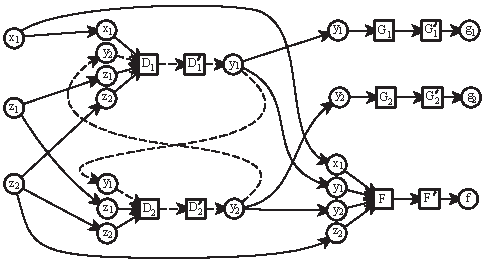
\includegraphics[width=.8\textwidth]{images/sellar_cycles}
      \caption{ Dependency graph for the Sellar problem. \label{fig:sellar_graph}}
    \end{center}\end{figure}

    In the original graph syntax, a single node is given for every variable. This holds true for the graph
    within OpenMDAO, with only one minor caveat. In the case of any hierarchical variables, such as arrays
    or VariableTrees, one variable node is created to represent the overall variable with additional nodes
    created if any specific sub-variable is referenced (e.g. some slice of an array or some child variable from a
    VariableTree). Figure \ref{fig:subvars} shows how the sub-variable nodes relate to their parent variables.

     \begin{figure}[!htb]\begin{center}
      xxxxxxx\\xxxxxxx\\xxxxxxx\\xxxxxxx\\xxxxxxx\\xxxxxxx\\
      \caption{ Example graph with child nodes for sub-variables \label{fig:subvars}}
    \end{center}\end{figure}

    By representing heirarchical data as a single node, we help keep the overall size of the graph manageable
    when large chunks of data are being communicated. However, if some small sub-set of that data needs to be
    used somewhere it is not correct to indicate a dependence on the entire chunk of data. So in this case, a
    single new node representing the sub-variable is created with its own dependence on the parent variable.
    This book keeping becomes particularly important for when the graph is used to calculate derivatives or
    manage the partitioning of distributed data.

    \subsection{Determining Execution Order}

    The OpenMDAO framework uses a dependency graph to determine component execution order and to
    drive the process of invalidation, which finds the minimum set of components that needs to
    be re-executed when a set of inputs change. (ref: last OpenMDAO paper.) A dependency graph
    can also identify cycles in the graph, and hence a cycle in the dataflow that must be resolved
    by a solver. Similarly, the graph can also be used to examine the potential for parallelism at
    a component level.

    \subsection{Relevant Variable Identification}
    Given the dependency graph for any problem, in order to set up a design optimization the user
    must first specify a set of design variables, objectives, and constraints. Using graph
    path finding algorithms, such as [insert network x algorithms we use here, with citations as we can find them].

    The determination of driver subgraphs is a capability that will be investigated in this paper.
    Consider an optimizer with n parameters, 1 objective, and m constraints. The relevant
    subgraph of this problem is the set of component disciplines and their variable connection that
    lie within the subgraph between the parameters and the constraints and objective. This subgraph
    contains the components that execute when the optimizer requests a function evaluation. It is
    also useful for setting up and solving the coupled derivative system when the optimizer requests
    a gradient evaluation. For calculation of the coupled derivative in adjoint mode, further
    efficiency can be gained by using the subgraph that includes just the portion of the graph
    between a single constraint and the parameters. Similarly for forward mode, the subgraph would
    include just the portion of the graph between a single parameter and the constraints/objective.

    \subsection{Cycle Detection}
    \subsection{Mixed Analytic and Finite Difference Gradients}
    \subsection{Gradient Assembly}

  \section{CADRE Problem Formulation}

  \section{CADRE Results}

The OpenMDAO implementation of the CADRE problem was executed on a Macbook Pro (2.3 Ghz Core i7 processor, 4GB 1600 Mhz DDR3 memory, running OSX 10.8.5)
over the course of two days, to a termination tolerance of $10^{-5}$. This tolerance
was achieved within approximately 106 iterations, using the SNOPT\cite{gill2005snopt}
optimizer.

\begin{figure}
\centering
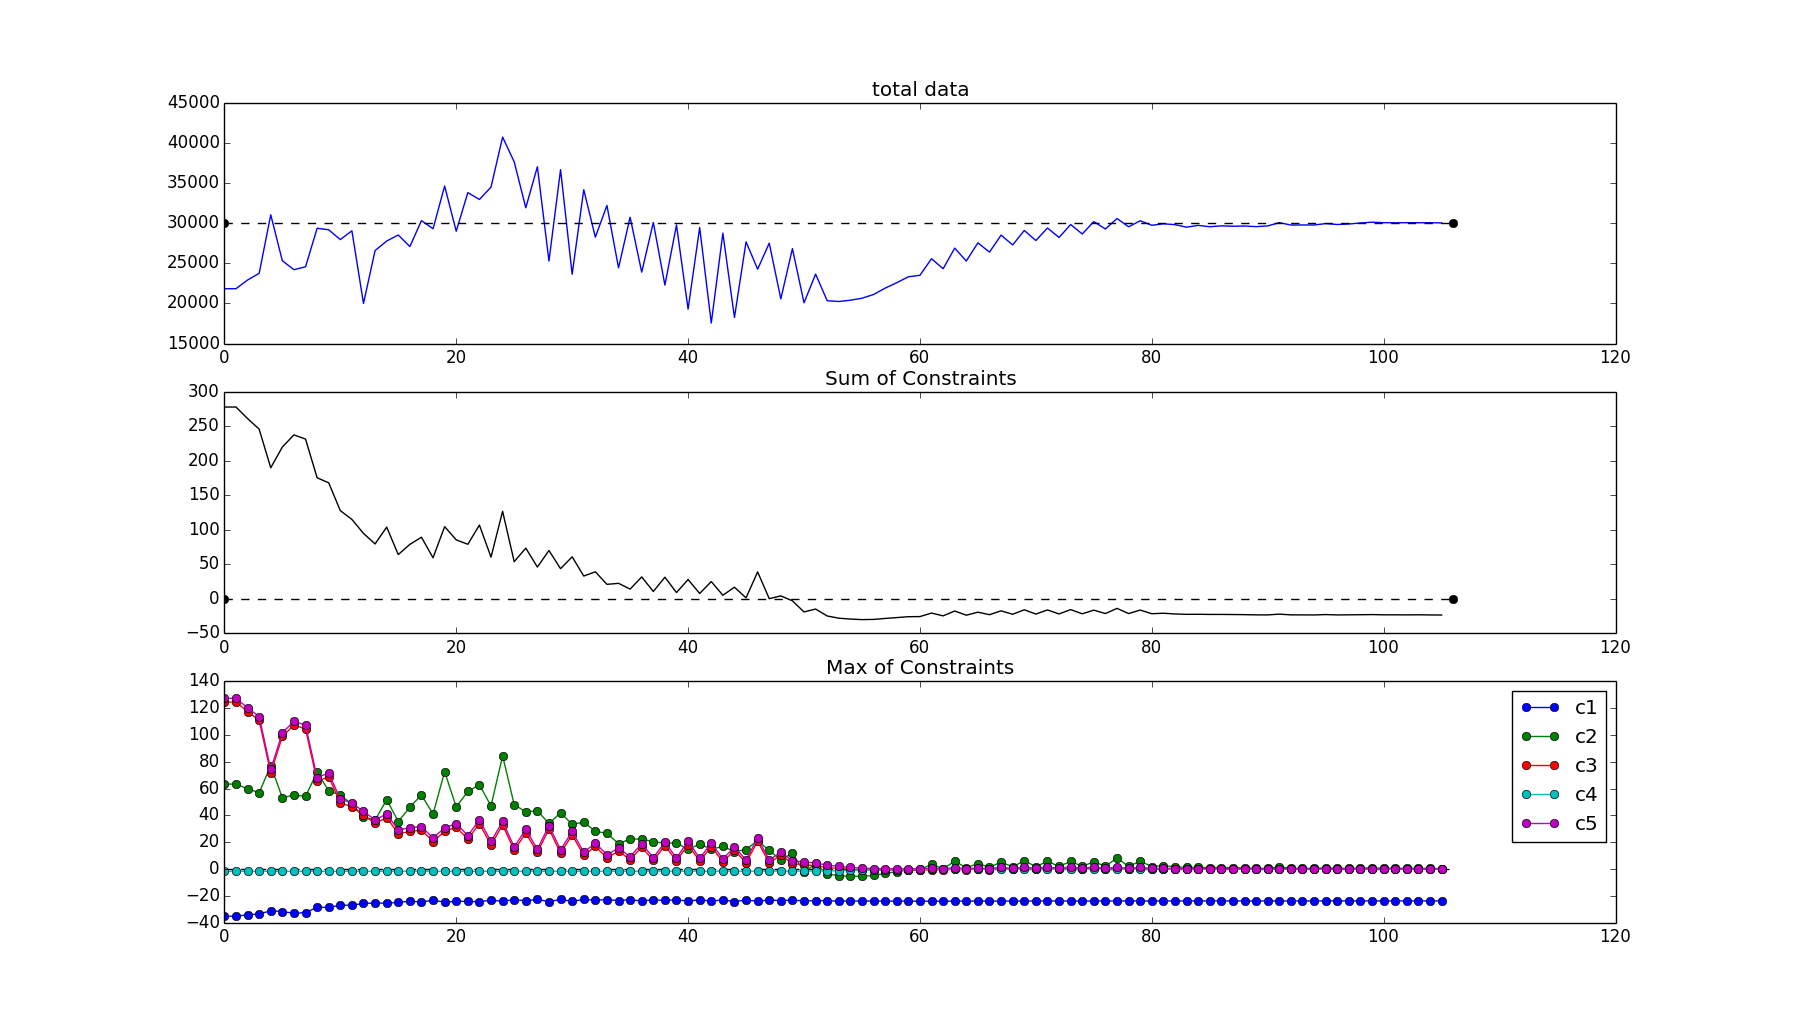
\includegraphics[width=0.99\textwidth]{images/opt.png}
\caption[width=0.22\textwidth]{Convergence of the CADRE problem.}
\label{convergence}
\end{figure}


Figure \ref{convergence} illustrates the convergence of the CADRE problem over the course of
these iterations. The first row plots the
value of the objective function, the total data downloaded over each design point. The objective
function oscillated greatly over the course of the first half of the computed iterations, but
stabilized by the 80th iteration near the value previously determined[cite CADRE paper]
to be the optimal design.

The second row plots the maximum value of each constraint across all design points at
each iteration. As all of the problem constraint are non-positive for a feasible design,
this can be taken as a cursory measure of overall problem feasibility.
The third row plots the maximum value of each constraint across each of the design points,
but separated according to specific constraint type. These two plots both indicate that the
oscillatory behavior of the objective function coincided with a steady decrease in design
infeasibility. Once a feasible state was reached (near the 50th iteration), the optimizer
began refining the design towards a more favorable value of the objective function.

\begin{figure}
\centering
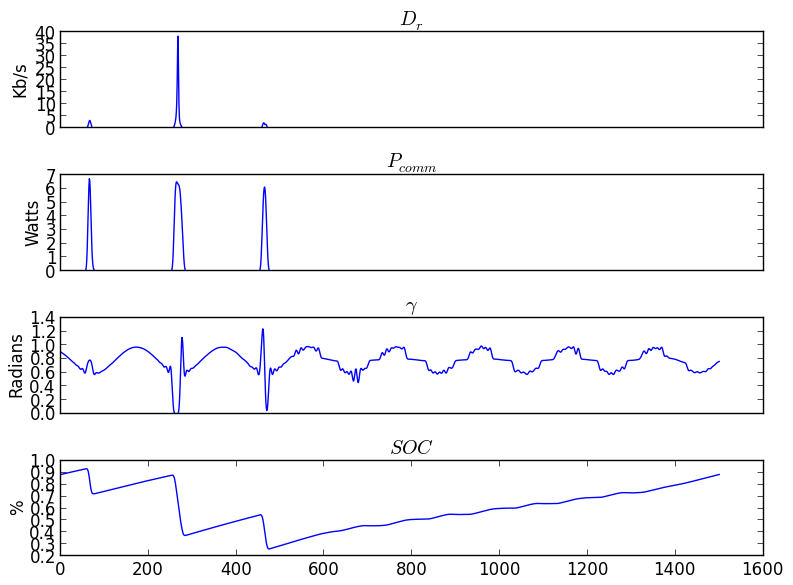
\includegraphics[width=0.8\textwidth]{images/pt_3_data.png}
\caption[width=0.4\textwidth]{Plots of the bit rate, communications systems power, craft roll angle,
and battery charge level over the half-day time period covered by the $4^{\textrm{th}}$ design point.}
\label{pt3_data_results}
\end{figure}

Figure \ref{pt3_data_results} shows plots of selected variables for the $4^{\textrm{th}}$ design point,
to illustrate the fidelity of the recovered solution. These variables are the communications bit rate ($D_r$), communications systems power level ($P_{comm}$), craft roll angle ($\gamma$),
and battery charge level ($SOC$). Prior to the optimization, these variables
were each instantiated to uniform values
(across all time points) of 0, 0, $\frac{\pi}{4}$, and 0 respectively. The optimizer, operating on
OpenMDAO's graph formulation of the problem succeeded at converging each of these variables to the values
shown, for each time point. Line of sight is seen to have been achieved in three short ranges of time near the
beginning of the modeled half-day design point. Interestingly, though the data rate achieved in the second
time period with affirmative line of sight is significantly higher than the other two periods, the optimizer
converged to a solution that provided power to the communications system near uniformly for each of these
three time periods.

Figure \ref{pt3_data_results} shows that the craft roll angle, $\gamma$, roughly approximates a sine function
with a wavelength of 90 minutes (the approximate orbital period of the satellite),
with short term perturbations during the time
periods where line of sight is gained with the ground station. That is, the optimizer successfully
converged to a solution with the satellite continuously turned to maximize exposure to the sun,
except when turning to point its antenna towards the ground station during times when
communication is possible. This dynamic is also reflected in the battery state of charge ($SOC$)
data plotting in the bottom row, with the battery losing charge quickly during
communication with the ground station, but recharging while tracking with the sun.

Further post processing of the data included automatic geographical rendering of the trajectories of
the CADRE satellite for each of the 6 design points, using the Google
Maps\footnote{http://developers.google.com/maps/} and Google
Earth\footnote{http://developers.google.com/earth/} APIs. The trajectories are
represented as polygonal chain ("polyline") elements, colored according to the
satellites communication bit rate with the ground station during the corresponding
window of time. Each colored line segment are centered on the locations
determined by the time points when the data bit rate values were calculated
by the OpenMDAO model.

Figure \ref{pt3_g_earth} communications bit rate along the trajectories of the
CADRE satellite during the $4^{\textrm{th}}$ design point. This can be compared
directly with Figure \ref{pt3_data_results}, where one large spike in communications
bit rate was preceded and then succeeded by two short time periods of lesser
data rates. Plotted geographically, this is seen to be due to the procession of
the satellites orbit, where the period of maximal data rate corresponds to a
pass of the satellite directly over the ground station location. The proceeding and
succeeding data rate spikes correspond to passes over the near Atlantic and
Rocky Mountain regions, respectively.


Figure \ref{allpt_flatmap} similarly shows trajectory and bit rate data plotted
from all six design points, centered on the United States. The orbital passes
that are close enough to the ground station for communications can all be seen.
Figure \ref{allpt_g_earth} zooms this view out to show coverage of the trajectories
of all design points across the Earth.


\begin{figure}
\centering
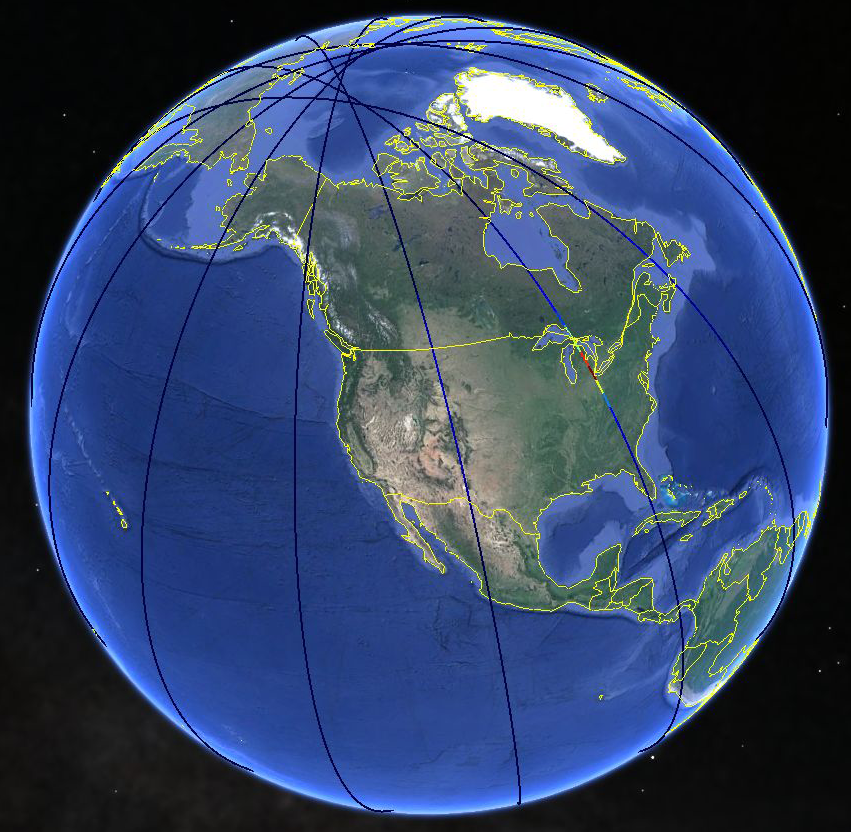
\includegraphics[width=0.8\textwidth]{images/pt3_gearth3.png}
\caption[width=0.4\textwidth]{Plot of the trajectories of the CADRE satellite
for the $4^{\textrm{th}}$ design point onto the surface of the Earth, illustrating the
communication data rates near the ground station.}
\label{pt3_g_earth}
\end{figure}


\begin{figure}
\centering
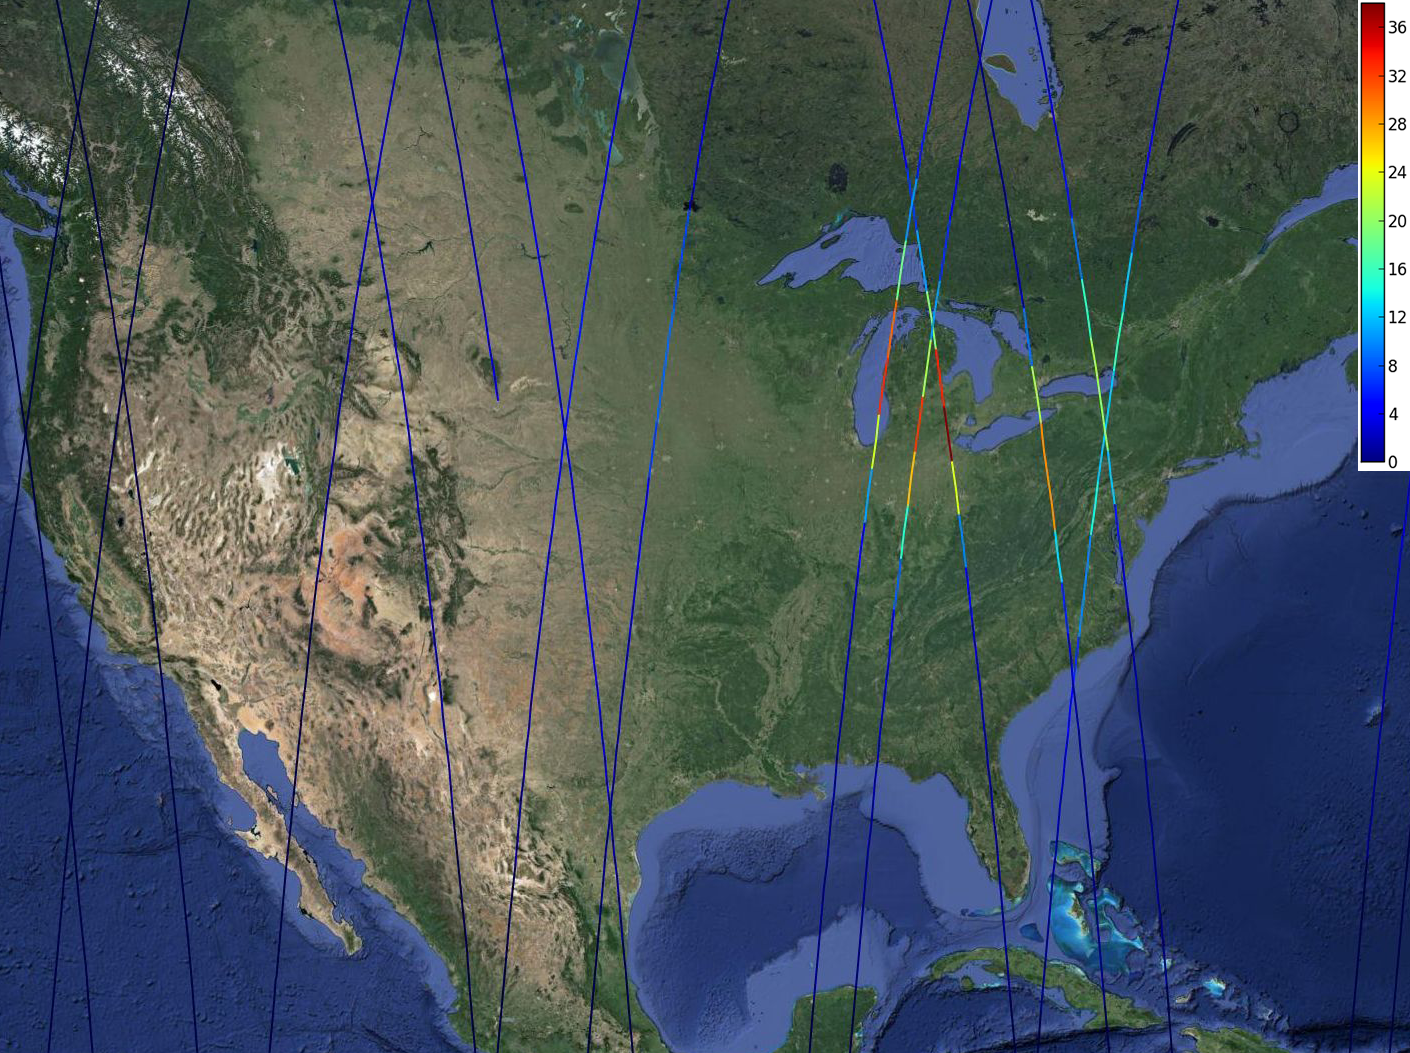
\includegraphics[width=0.8\textwidth]{images/allpts_map_data.png}
\caption[width=0.4\textwidth]{Plot of the trajectories of the CADRE satellite
for all 6 design points onto the surface of the Earth, illustrating the
communication data rates near the ground station.}
\label{allpt_flatmap}
\end{figure}


\begin{figure}
\centering
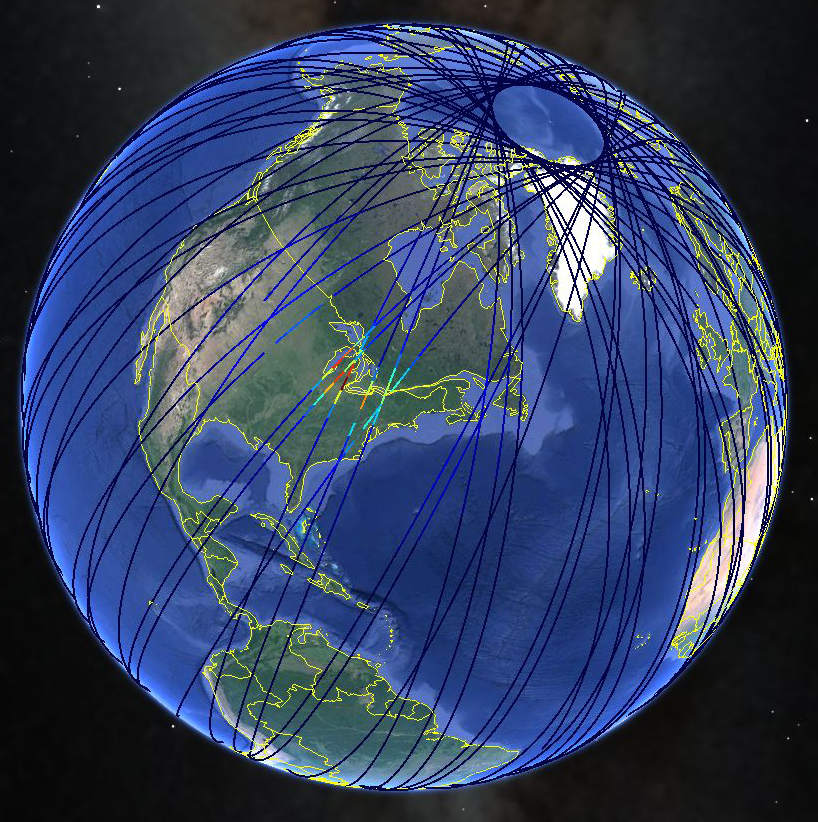
\includegraphics[width=0.8\textwidth]{images/allpts_gearth2.png}
\caption[width=0.4\textwidth]{Plot of the trajectories of the CADRE satellite
for all 6 design points onto the surface of the Earth.}
\label{allpt_g_earth}
\end{figure}


  \section{Aero-Structural Problem Formulation}

  \section{Aero-Structural Results}

  \section{Conclusion}

  \bibliography{references}


\end{document}
